\documentclass[11pt, a4paper]{article}

\usepackage[T1]{fontenc}
\usepackage[utf8]{inputenc}
\usepackage[polish]{babel}
\usepackage{listings}
\usepackage{mathtools}
\usepackage{blindtext}
\usepackage{scrextend}
\usepackage{graphicx}


\graphicspath{ {./images/} }


\begin{document}

\title{MOwNiT\\Laboratorium 3}
\author{Kacper Janda}
\date{}
\maketitle

\section{Wady klasycznego algorytmu Gaussa}
Rozwiązywanie układu równań liniowych podstawową metodą Gaussa zawodzi gdy na przekątnej macierzy A istnieją zera. Algorytm próbuje wtedy podzielić przez \begin{math} 0 \end{math} co prowadzi do błędu. Algorytm ten nie uwzględnia postaci macierzy A - gdy jest ona macierzą diagonalną algorytm i tak wykonuje wszystkie operacje. Metoda ta posiada złożoność obliczeniową \begin{math} O(n^3) \end{math}. Kolejnym problemem jest fakt powstawania błędów numberycznych spowodowanych dzieleniem przez liczby o małej wartości. Ma to znaczny wpływ na wynik w szczególności w przypadku macierzy źle uwarunkowanych.\\

\section{Optymalizacja algorytmu Gaussa}
Aby zmniejszyć czas potrzebny rozwiązywania układu równań można zastosować rozkład LU macierzy A. Zmniejsza to złożoność obliczeniową o stały współczynnik. Innym sposobem na poprawienie działania algorytmu jest zastosowanie wybierania elementów głównych. Pozwala to zredukować błędy numeryczne.\\

\section{Porównanie wydajności}
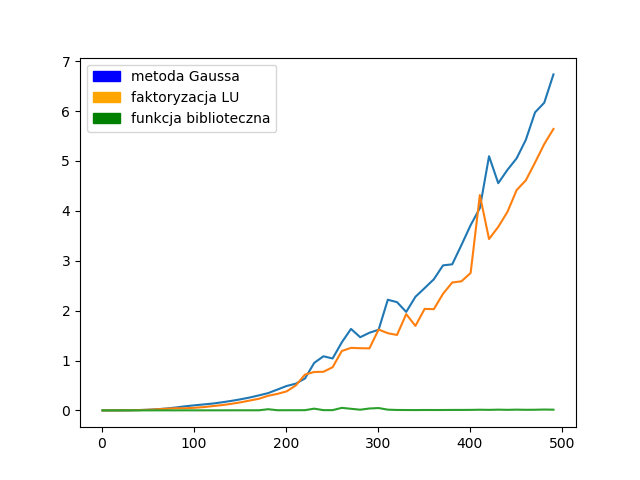
\includegraphics[scale=0.8]{Figure_1}

Wykras pokazuje, że w celu uzyskania jak najlepszej wydajności należy korzystać z funkcji bibliotecznych (w tym przypadku została wykorzystana funkcja 'solve' z biblioteki 'numpy.linalg'). Zgodnie z przewidywaniami wykresy zaimplementowanych funcji przedstawiają złożoność \begin{math} O(n^3) \end{math}

 

\end{document}